% Section content template for individual Educative lessons
% This file contains the actual content for a specific section
% Generated from Educative API section content

% Section: System Design: Distributed Logging
% Section ID: 6747547922333696
% Section Slug: system-design-distributed-logging
% Generated: 2025-12-07T22:00:33.619909

\subsection{Logging}\label{22oY2aHilArgNtYO-S-NA}
\\
A \textbf{log file} records details of events occurring in a software application. The details may consist of microservices, transactions, service actions, or anything helpful to debug the flow of an event in the system. Logging is crucial to monitor the application's flow.

\begin{figure}[htbp]
 \centering
 
\includegraphics[width=0.15\textwidth]{Images/chapter_22/section_6747547922333696/4628299206492160.png}
 
\end{figure}

\subsection{Need for logging}\label{cuSivbmhuS6O_aiI3poBe}
\\
Logging is essential in understanding the flow of an event in a distributed system. It seems like a tedious task, but upon facing a failure or a security breach, logging helps pinpoint when and how the system failed or was compromised. It can also aid in finding out the root cause of the failure or breach. It decreases the meantime to repair(Mean time to repair (MTTR) is a basic measure of the maintainability of repairable items. It represents the average time required to repair a failed component or device. (Source: Wikipedia)) a system.
\\
Why don't we simply print out our statements to understand the application flow? It's possible but not ideal. Simple print statements have no way of tracking the severity of the message. The output of print functions usually goes to the terminal, while our need could be to persist such data on a local or remote store. Moreover , we can have millions of print statements, so it's better to structure and store them properly.

\begin{figure}[htbp]
 \centering
 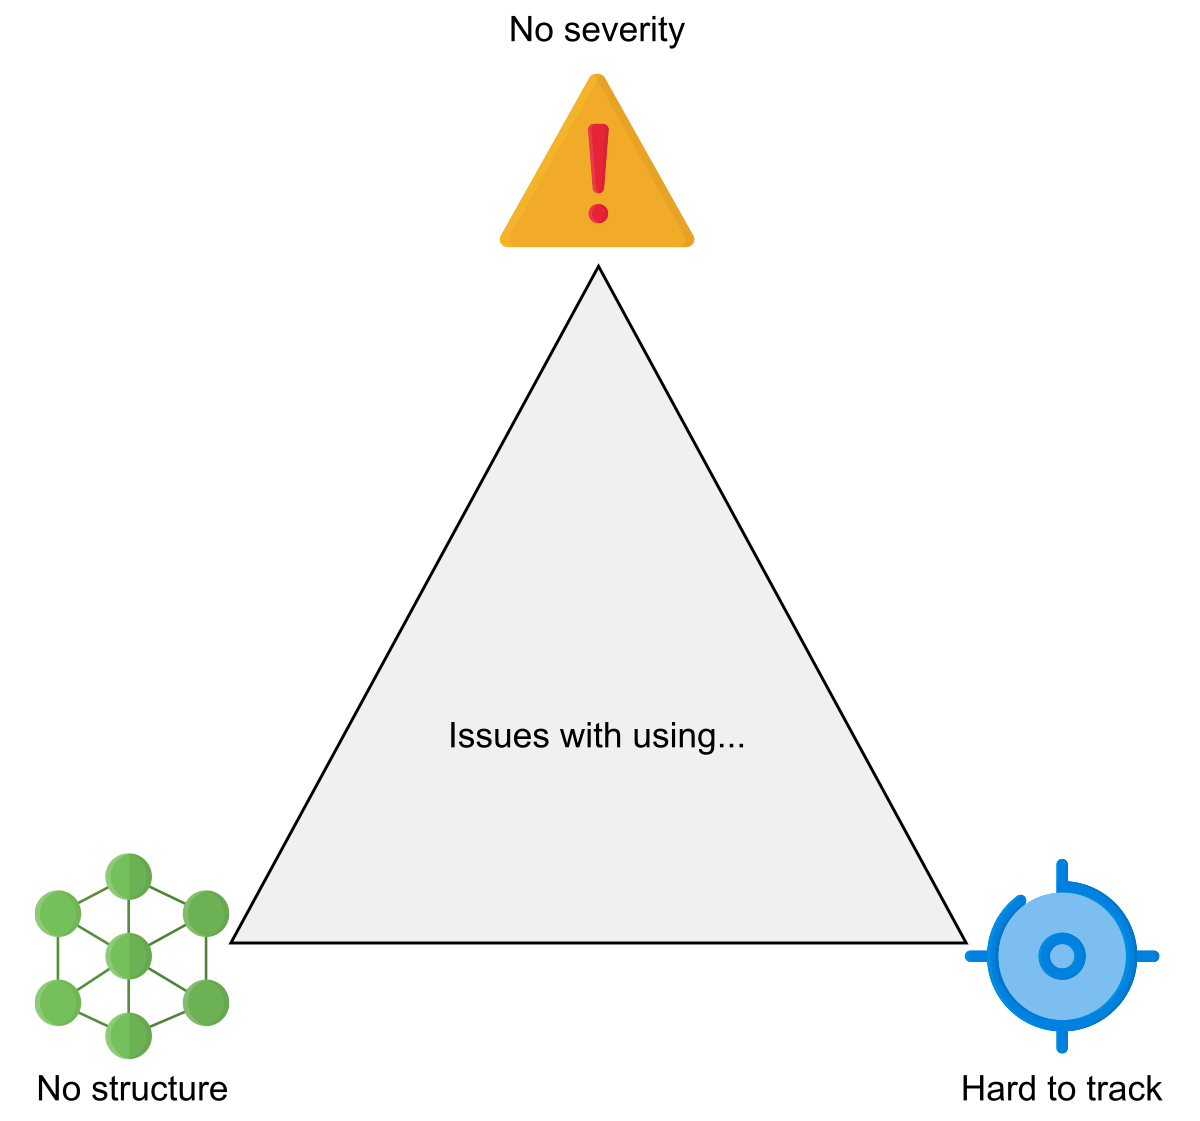
\includegraphics[width=0.25\textwidth]{Images/chapter_22/section_6747547922333696/6199989915353088.png}
 \caption{Issues with using print statements as an alternative to logging}
\end{figure}

Concurrent activity by a service running on many nodes might need causality information to stitch together a correct flow of events properly. We must be careful while dealing with causality in a distributed system. We use a logging service to appropriately manage the diagnostic and exploratory data of our distributed software.
\\
Logging allows us to understand our code, locate unforeseen errors, fix the identified errors, and visualize the application's performance. This way, we are aware of how production works, and we know how processes are running in the system.
\\
Log analysis helps us with the following scenarios:

\begin{itemize}
\item
\protect\phantomsection\label{h6rBn3OLIBVqiHZ1wPu3d}
To troubleshoot applications, nodes, or network issues.
\item
\protect\phantomsection\label{5puQ0Vxv3lcdKebQGiBjJ}
To adhere to internal security policies, external regulations, and compliance.
\item
\protect\phantomsection\label{QXCx5l3ktRilrhSBh-5QR}
To recognize and respond to data breaches and other security problems.
\item
\protect\phantomsection\label{eMaexbJDgdrIQk-7ZgyKn}
To comprehend users' actions for input to a recommender system.
\end{itemize}
\\
What are some security concerns to consider when designing a distributed logging system? How would you mitigate them?
\\
Write your answer in the widget below.

\textbf{Question:}

Security in Distributed Logging System

\textbf{Reference Answer:}

Concern: Sensitive data exposure Mitigation: Avoid logging personally identifiable information (PII) or sensitive data. If logging is necessary, mask or encrypt sensitive fields to prevent misuse.
\\
Concern: Unauthorized access to logs Mitigation: Implement strong authentication and fine-grained authorization controls to restrict log access only to trusted users or systems.
\\
Concern: Logging system vulnerabilities Mitigation: Harden the logging infrastructure by securing endpoints, applying regular patches, and enforcing least-privilege access.
\\
Concern: Unsecured log transmission or storage Mitigation: Encrypt log data both in transit and at rest to protect against eavesdropping or data breaches.
\\
Concern: Lack of visibility into logging system misuse Mitigation: Conduct regular audits and enable monitoring to detect anomalies, unauthorized access, or suspicious activity within the logging pipeline.

\subsection{How will we design a distributed logging system?}\label{6FBys8A3TarKhwr5TDugN}
\\
We have divided the distributed logging system design into the following two lessons:

\begin{enumerate}
\item
\protect\phantomsection\label{CbO9xxSOz7hMrRlvLwqgq}
\href{https://www.educative.io/courses/grokking-the-system-design-interview/introduction-to-distributed-logging}{\textbf{Introduction}}: We'll discuss how logging works at a distributed level. We'll also show how we can restrict the huge size of a log file, and structure them. This lesson will guide us about the requirements we should consider while logging information about a system.
\item
\protect\phantomsection\label{92-23NUG5JJ4TOp6aod0k}
\href{https://www.educative.io/courses/grokking-the-system-design-interview/design-of-a-distributed-logging-service}{\textbf{Design}}: In this lesson, we'll define the requirements, API design, and detailed design of our distributed logging system.
\end{enumerate}

% End of section content